\documentclass{styles/llncs}

\usepackage[whole]{bxcjkjatype}
\usepackage{pgfplotstable}
\let\proof\relax
\let\endproof\relax
\usepackage{amsthm}
\usepackage{pifont}
\usepackage{balance}
\usepackage{times}
\usepackage{xspace}
\usepackage{textcomp}
\usepackage[font=small, skip=1pt]{caption}
\usepackage[hyphens]{url}
\usepackage[breaklinks=true,
            hidelinks,
            hyperindex,
            colorlinks = true,
            linkcolor = blue,
            urlcolor  = blue,
            citecolor = blue,
            anchorcolor = blue]{hyperref}
% \usepackage{listings, multicol}
%\usepackage{enumitem}

\colorlet{light-gray}{gray!20}
\definecolor{lightgray}{rgb}{.9,.9,.9}
%--------------------------
%\usepackage{epsfig,endnotes}
\usepackage{graphicx}
\usepackage{color}
\usepackage{pgfplotstable}
\usepackage{makeidx}
\usepackage[justification=justified]{caption}
\usepackage[justification=justified]{subcaption}
\usepackage{tikz}
\usepackage{environ}
\usepackage{amsthm}
\usepackage{pifont}
\usepackage{cite}

\usetikzlibrary{calc}
\usetikzlibrary{patterns}
\usetikzlibrary{shapes.multipart, arrows}
\usetikzlibrary{decorations.pathreplacing}
\usetikzlibrary{positioning, backgrounds}

\usetikzlibrary{
    shapes.geometric,
    positioning,
    fit,
    calc,
    shapes.multipart
}
\usetikzlibrary{arrows,automata,positioning}


\usepackage{pgfplots}
\usepackage{amssymb}
\usepackage{amsmath}
\usepackage{multirow}
\usepackage{relsize}
\usepackage{xcolor,colortbl}
\captionsetup{compatibility=false}
\usepackage{algorithm,algpseudocode}
\usepackage{algorithm,algpseudocode}
\usepackage{enumitem}
\usepackage{courier}
\usepackage{listings, multicol}
\usepackage[justification=centering]{caption}
\usepackage{framed}
\usepackage{xspace}
\usepackage{tablefootnote}
\usepackage{footnote}
\usepackage{color}
\usepackage{etoolbox}
\usepackage{array}
\newcolumntype{L}[1]{>{\raggedright\let\newline\\\arraybackslash\hspace{0pt}}m{#1}}
\newcolumntype{C}[1]{>{\centering\let\newline\\\arraybackslash\hspace{0pt}}m{#1}}
\newcolumntype{R}[1]{>{\raggedleft\let\newline\\\arraybackslash\hspace{0pt}}m{#1}}


\makeatletter
\pretocmd{\chapter}{\addtocontents{toc}{\protect\addvspace{15\p@}}}{}{}
\pretocmd{\section}{\addtocontents{toc}{\protect\addvspace{10\p@}}}{}{}
\pretocmd{\subsection}{\addtocontents{toc}{\protect\addvspace{5\p@}}}{}{}
\makeatother
% \usepackage{refcheck}

\makesavenoteenv{tabular}
\makesavenoteenv{table}
\newcolumntype{C}[1]{>{\centering\arraybackslash}p{#1}}

\newcommand{\para}[1]{\noindent \textbf{#1}}
\newcommand{\code}[1]{\texttt{#1}}
\newcommand{\var}[1]{\texttt{#1}}
\newcommand{\fun}[1]{\textit{#1}}
\newcommand{\codename}{{\scshape Gormos}\xspace}
\newcommand{\cmark}{\ding{51}}
\newcommand{\xmark}{\ding{55}}
\newcommand{\send}[2]{{#1}~$\rightarrow$~{#2}}

\newcommand{\todo}[1]{\textcolor{green} {LL: #1}}
\newcommand{\eg}{{e.g.,}\xspace}
\newcommand{\ie}{{i.e.,}\xspace}
\newcommand{\mtt}[1]{{\mathtt{#1}}\xspace}
\setlength{\belowcaptionskip}{-10pt}

\newcommand{\sspace}{\vspace{-7pt}}
\newcommand{\ssspace}{\vspace{-3pt}}
\pagestyle{plain}
\graphicspath{{./images/}}
\begin{document}

\title{
  \codename: A high performance and scalable design for decentralized applications
}
\author{
    Loi Luu, Yaron Velner, Alex Xiong\\
    \email{\{loiluu, yaron, alex\}@kyber.network}
}
\institute{Working draft, last updated \today}

{\def\addcontentsline#1#2#3{}\maketitle}

\section*{Abstract}

We introduce \codename, the first protocol design for a high performance decentralized applications that allows high frequency interactions, low latency settlement and great interoperability. \codename is built on top of various technologies, including Plasma~\cite{plasma} and our previous work on sharding~\cite{elastico} and PeaceRelay~\cite{peacerelay}. The protocol theoretically allows for asymptotically optimal scaling up to millions of transactions per second, without compromise on security and decentralization. While this paper describes \codename in the context of decentralized exchanges, the approach can be applied to various other applications like gaming, payments, social networks and so on.

\setcounter{tocdepth}{2}
\tableofcontents
\newpage
\section{導入}
\label{sec:intro}

Ethereumは、2015年の導入以来、プロジェクトや企業がネットワーク上で分散アプリケーションを立ち上げることに大きな関心を集めています。その結果、たとえばトークンの大量販売やCryptokittiesのようなゲームなどにより、Ethereumネットワークは過去に何度かのトランザクション詰まりがありました。そのような場合、ユーザーは取引を送信するためにはるかに高い手数料を支払うか、取引を確認するまで何時間も待たなければなりません。 Bitcoinのトランザクションのピークは、1日あたり約425,000件~\footnote{\url{https://blockchain.info/charts/n-transactions?timespan=all}}、Ethereumのトランザクション数は140万件~\footnote{\url{https://etherscan.io/chart/tx}}で、これは1億5000万人を超えるアクティブユーザーを抱えるTwitterや、ユーザー数14億人のFacebookに比べてはるかに少ない数です。さらに、Ethereumでの平均ブロック待ち時間が15秒になると、ほとんどのユーザーにとって使用可能なプラットフォームを構築する上でより多くの課題が生じます。スケーラビリティとレイテンシの両方の制約は、分散アプリケーションが主流になるのを困難にします。

分散型取引所を例に挙げてみましょう。既存の分散型取引所は、流動性が低く、ユーザーエクスペリエンスが低く、スケーラビリティが低い(インフラストラクチャのため)などの大きな問題があります。これらの課題に取り組むにはさまざまな提案がありますが、各ソリューションはセキュリティ、分散化、またはサポート機能のいずれかで大きな妥協を見せています。たとえば、現在のKyberNetworkの取引所では、完全にオンチェーンで実行することで最適なセキュリティを実現し、わずかなクリックでより良いユーザーエクスペリエンスを実現し、取引を完了することができますが、リミットオーダー、トレーディングレバレッジ、または高頻度取引はまだサポートできません。0x~\footnote{\url{https://0xproject.com/}}やEtherDelta~\footnote{\url{https://etherdelta.com/}}のような他の取引所は、ハイブリッドモデル、すなわちオフチェーンの(集中化された)注文帳を持ち、チェーン上の決済を行うことによって、集中取引所での取引経験をシミュレートしようとします。ユーザーは本質的に注文書を保管して提供するサーバー/ウェブサイトに頼らざるをえないため、明確なセキュリティのトレードオフが存在します。いずれの解決策もEthereumブロックチェーン上で1つのオンチェーン取引を行うため、スケーラビリティの制約と待ち時間の長い決済が問題になります。執筆時点では、レイテンシは平均で約15秒であり、Ethereumブロックチェーンはトランザクションタイプに応じて毎秒約10-15回のトランザクションを処理できます。さらに、ブロックチェーンがCryptokittiesやいくつかの重要な公開トークンの販売などのイベントで混雑する際に、トランザクションのガス支払いにもっと高い取引手数料を支払わなければならないかもしれません。そのようなソリューションは、明らかに、Binance~\footnote{\url{https://www.binance.com/}}やHuobi~\footnote{\url{https://www.huobi.pro/}}などの集中化された取引所と競争することができません。現在のレポートでは~\cite{binance-report}、Binanceはピーク時に毎秒40,000リクエストを処理すると主張し、すべての分散型取引所のパフォーマンスを大きく引き離しました。重要な設計上の変更がない場合、分散された変更はほんの一部でしか使えず、プロのトレーダーは言うまでもなく主流のユーザーを引き付けることはできません。

最近、Plasmaは、別のブロックチェーンにトランザクションをプッシュし、ユーザーを重要なブロックチェーンバリデーターから保護するためにクリプトエコノミクスを使用し、頼もしいスケーラビリティを持ってこの問題を助けにきました~\cite{plasma}。しかし、既存のPlasma設計は高レベルであり、分散型取引所には最適化されていません。 Plasmaのスケーリングは、Plasmaバリデーターの物理的容量によっても制限されます。したがって、ユーザーエクスペリエンスとセキュリティーの保証を損なうことなく、最適なスケーリングを提供しません~\footnote{正確には、Plasmaのホワイトペーパーには、Plasmaの子チェーンという概念があります。 技術的には無限のスケーラビリティを提供しますが、資産を多くのレイヤーにわたって移動する必要があるため、ユーザーエクスペリエンスのコストがかかります。 Plasmaの子チェーンは、セキュリティ保証のトレードオフのもう1つのレイヤーです。}。Binanceの規模を実現するとなると、各Plasmaノードは、テラバイトのデータとネットワーク帯域幅を格納しなければならない場合があります。 それにかかわらず、Plasmaに関しては相互運用性に関して議論されていない。

スケーラビリティは、分散取引所だけでなく、ソーシャルネットワーク、ゲームなどの他の多くのアプリケーションにとっても明らかに問題です。たとえば、Etheremon~\footnote{\url{https://etheremon.com}}とPeepeth~\footnote{\url{https://peepeth.com}}は現在、より良いユーザービリティを提供するために複数のアクティビティを束ねてチェーンにコミットするというトレードオフを採用しています。まだコミットされていないアクティビティはプロジェクトサーバ内にローカルに保存されているため、システムのセキュリティが大幅に低下します。

本稿では、低レイテンシの安全でスケーラブルなブロックチェーンのための新しいプロトコル設計である\codenameを紹介します。上位レベルでは、\codenameはPlasmaとShardingの間のスウィートスポットを見つけ出します。これにより、i) ブロック時間がはるかに短くても安全にサイドチェーン上でトランザクションを実行できるようにし、 ii)ネットワーク内のノードまたはバリデーターから多くのリソースを必要とすることなく、線形スケーリングを可能にします。 \codenameは一般的な設計ではなく、異なるコンポーネントを持ち、互いに相互作用することはめったにない種類のアプリケーションに対してのみ有効です。たとえば、分散型取引所の場合、各取引ペアを取引所の1つの構成要素と見なすことができ、異なる取引ペアの間の取引は、通常の取引ペアでの取引よりもはるかに少ないとみなすことができます。したがって、分散化された取引に対してシャーディングを効率的に適用して、ワークロードを異なるシャードに分散し、より高いスケーラビリティを達成することができます。さらに\codenameは、その設計における相互運用性、すなわちBitcoin、Litecoin、ETC、または異なるブロックチェーンからの暗号通貨をPlasmaチェーンに移すことも考慮に入れています。同様に、\codenameはEtheremonやPeepethのようなアプリケーションにも適用でき、ユーザーエクスペリエンスを犠牲にすることなく、より良いセキュリティ保証を提供します。

本稿では理解を容易にするために、以降の節では分散型取引所の文脈で\codenameについて説明し、~\ref{sec:others}項にて他のアプリケーションに適用する方法について述べます。

\subsection{望まれる性質}
最先端のさまざまな分散取引所の事例や、KyberNetworkのリリース後数ヶ月にわたってユーザーから得られたフィードバックから、高性能な分散型取引所(DEX)の望ましい特性を次のようにまとめます。

\begin{itemize}
\item \textbf{スケーラビリティ}. DEXは、DEXのバリデーター(またはノード)からの重要なハードウェアおよびネットワーク帯域幅を必要とせずに、毎日何百万人ものユーザーが取引できるようにする必要があります。 さらに、いくつかの一般的な取引ペアがDEXのすべての能力を占める可能性があり、その結果、他のペアのユーザーの取引経験に影響を及ぼす可能性があります。 スケーラブルなDEXは、このような問題を防止し、ユーザーがすべてのユーザーのペアを円滑に交換できるようにする必要があります。
\item \textbf{低レイテインシ}. DEXは待ち時間の短い取引、すなわち注文が提出されてから確認されるまでの時間をミリ秒単位ではないとしても数秒にする必要があります。 私たちは、私たちのデザインで2秒の確認とインスタント決済を達成することを目指しています。
\item \textbf{セキュリティと非中央集権性}. これは、DEXの基本的な特性であり、人々が中央集権的取引所よりもDEXを好む理由です。非中央集権は、DEXにおいて特に重要です。なぜなら、より良い透明性と検閲に抵抗する取引の需要が大きいからである。 最近、中央集権的取引所がどのように透明であるかについての疑問が投げかけられています~\footnote{\url{https://medium.com/@sylvainartplayribes/chasing-fake-volume-a-crypto-plague-ea1a3c1e0b5e},\newline \url{https://cointelegraph.com/news/okex-resolves-futures-price-slip-impact-as-trader-threatens-suicide}}。
\item \textbf{相互運用性}. DEXは、Bitcoin、Ethereum、Litecoin、Ethereum Classic、EOSなどを含む、これらに限定されない異なる暗号通貨を取引できるようにすべきです。 これは、他のプロパティを妥協することなく行う必要があります。
\end{itemize}
これらは、中央集権的取引所と競争できるようにするためにDEXが持たなければならない主な望ましい特性です。 高い流動性、優れたユーザーエクスペリエンスなどを含む展開と採用に関しても重要な非プロトコルの理想的な特性があります。しかし、これらの特性は、我々が構築している高性能な分散型交換を構築する主な問題とは正反対です。

\section{関連プロジェクト}
\textbf{なぜPlasmaチェーンのツリー構造を用いないのでしょうか?}慎重な読者は、\codenameとPlasmaチェーンのツリー構造との違い、すなわち既存のPlasmaチェーンの上に別の子Plasmaチェーンを有することとの違いが何であるか疑問に思うかもしれません。それは、PlasmaがLayer-2のレイヤー2であるから、すなわち、ルートチェーンの上に別個の層を形成するからです。一般に、レイヤー2のソリューションにはある種のセキュリティのトレードオフがあります。たとえば、Plasmaユーザーは、何か悪いことが起こっていないかどうかを確認し、手遅れになる前にexitをする必要があります。 Plasmaチェーンの上にレイヤー2のソリューションを増やすことで、よりセキュリティのトレードオフが導入され、ユーザーのフォローが難しくなります。また、開発者は、プラットフォームを構築するか、プラットフォームのセキュリティ保証について理由を判断することも難しくなります。一方、シャーディングは、セキュリティの妥協をせずにコンセンサス層でスケーラビリティを提供します。シャーディングの主なトレードオフは、クロスシャードトランザクションによるユーザービリティです。しかし、\codenameでは、ネットワークを異なる取引ペアごとに異なるシャードに分割し、クロスシャード取引の量を最小限に抑える明確なロジックがあります。

\textbf{Zilliqaのような既存のシャーディングチェーンはどうでしょうか? } Zilliqaがシャーディングを使用してスケーラブルなブロックチェーンを構築しているため、Zilliqaの上にプラットフォームを構築しない理由が不思議に思うかもしれません。 主な違いは、Zilliqaはステートシャーディングをサポートしておらず、分散型取引のプラットフォームやその他のアプリケーションには最適化されていません。 何十億ものトランザクションを処理する際のストレージと状態の更新の要件は、ストレージ、帯域幅、および計算リソースの追加のコストをZilliqaで必要とします。 一方、\codenameは、状態処理、取引活動、および保管を明確に分離しています。 また、Plasmaを活用して、シャード内のバリデーターセットの数を減らし、トレーディングプラットフォームのレイテンシを短くします。

\textbf{Atomic Cross-Chain Swap (ACCS).}~\cite{atomic-swap-wiki}は、最も初期に考案されたシンプルなクロスチェーン取引の設計の1つで、以前にコミットされたハッシュの元データを明らかにすることによって払い戻しが可能な、nLockTimeによるコントラクトも用いる手法です(正式な記述はTesseract ~\cite{tesseract}のセクション2にあります)。ACCSの主な問題は3つあります。第1に、タイムロックの導入によってリアルタイムの交換が難しくなってしまったことによる高いレイテンシです。これは基本的に\textit{fair exchange problem}\cite{fair-exchange-impossibility}の結果です。第2に、複数のタイムロックを並行運用するマルチパーティACCSの文脈では、複雑さのためスケーラビリティが劣ります。第3に、注文の発見の遅延と流動性の課題です。それと比較して、\codenameは他の暗号化された通貨をトークン化し、相互運用性に対する複雑なアプローチを大幅に削減します。 \codenameは、それ自体でクロスチェーン転送で長い待ち時間を解決するわけではありません。しかし、いったんペッグされたトークンは、他のトークンと同様に簡単に取引され、\codenameで確定したものと見なされます。

\textbf{Payment ChannelやState Channel.}\cite{lightning, miller2017sprites} は、Blockchainからロック状態の預金を介してトランザクションをオフロードし、最終的には更新された状態でチェーンを解決する仕組みです。 特に、最近公表された\textit{generalized state channel}は、ブロックチェーンにブロードキャストすることなく、新しい機能をインストールするための反証的にインスタンス化された契約を利用します~\cite{Coleman2018, Dziembowski2018}。 ブロックチェーンのスループットを効率的に調整する一方で、DEXのようなアプリケーションでは、州内の参加者をチャンネルに誘導するだけで、グローバルオーダーブックを構築することはほとんど不可能です。


\section{デザイン}

私たちの設計のほとんどは、Plasma~\cite{plasma}の既存の作業とシャーディング~\cite{elastico}の以前の作業、ブロックチェーンの相互運用性~\cite{peacerelay}を活用しています。 私たちの目標は、前述のすべての望ましい特性を、セキュリティと分散化を最小限に抑えて達成することです。


\begin{figure}[t]
  \centering
  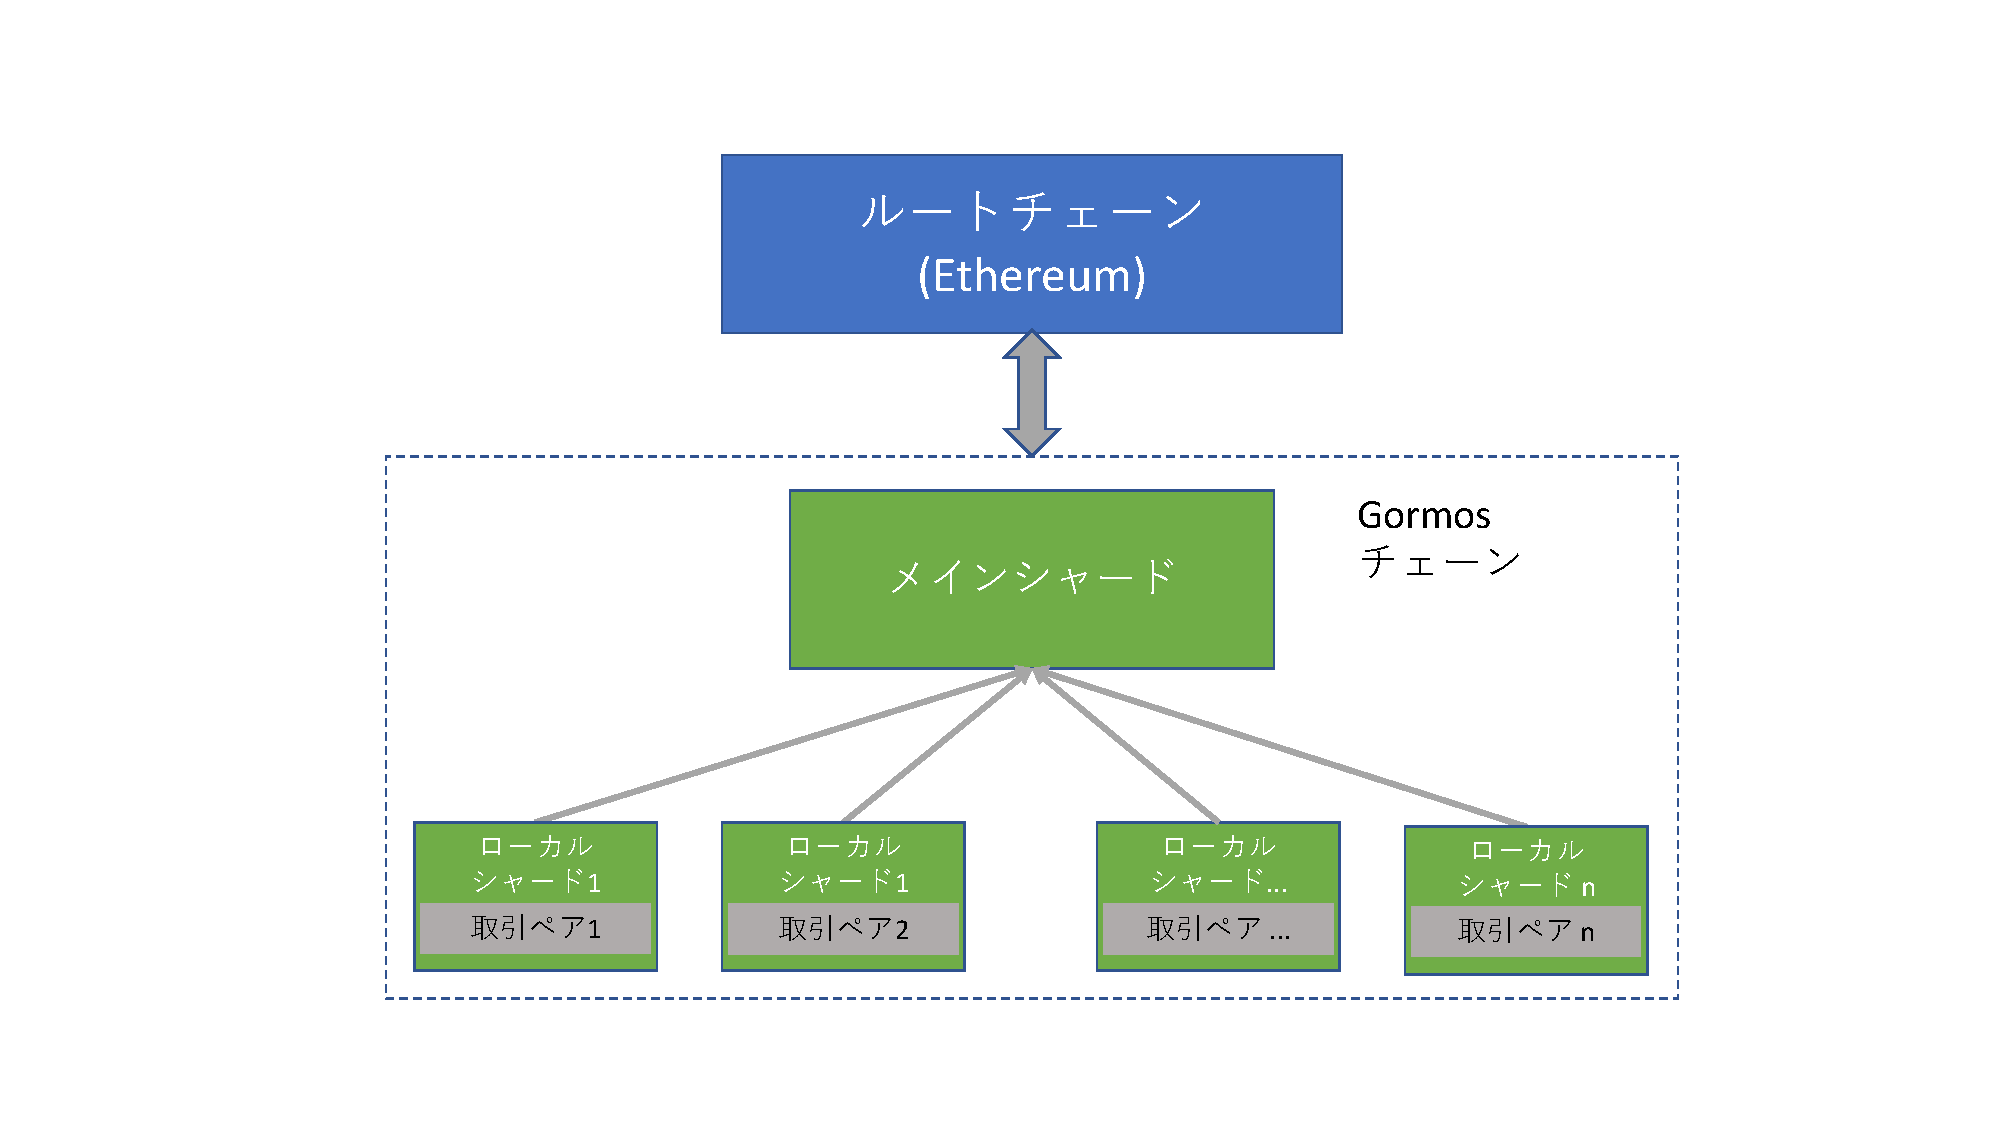
\includegraphics[width=0.8\textwidth]{images//architecture}
  \caption{\codename システムアーキテクチャ}
  \label{architecture}
\end{figure}


\subsection{デザインの概要}

\codenameの高レベルのデザインはFig.\ref{architecture}に示されています。 \codenameは、Plasmaとシャーディングの両方の素晴らしい技術を採用しています。 シャーディングアーキテクチャが組み込まれたこのPlasmaベースのアプローチでは、既存の取引プラットフォームにスケーリングの負荷を加えずに\footnote{より正確には、メインシャードにおいて漸近的に最適な(すなわち、一定のコストで)トークンペアやシャードを増加させることにより、より多くのユーザーの参加による計算コストやコミュニケーションコストの増加に対応します}、無限の取引ペアをリストすることができます。

私たちは新しいチェーンのバリデーターの中でビザンチン合意を採用して、低レイテンシとより迅速なファイナリティを達成しています。さらに重要なことに、このPlasmaチェーンの上にシャーディングアーキテクチャを設計して、無限のスケーリングを可能にします。私たちの調査では、異なる取引ペアのアクティビティを明確に分離し、異なるシャードにローカライズできます。たとえば、ETH / KNCとBTC / OMGとの間の取引は分離することができ、ETH / KNC間で取引するユーザーは、BTC / OMGを取引するユーザーに影響を与えません。この設計では、既存のリスティングペアのパフォーマンスと取引のユーザー体験に影響を与えることなく、プラットフォームがより多くのトークンを扱う場合に、より多くのシャードを追加することができます。このような設計は、多数の取引ペアに拡張することができ、毎秒数百万回の取引をサポートしますが、バリデーターのリソースの必要量は最小限に抑えられます。 \codenameのバリデーターは、状態全体を保管する必要もなく、プラットフォーム内で起こっているすべての取引を処理する必要もありません。代わりに、彼らは自分のシャードの状態を保存し、シャードに記載されている対応する取引ペアのすべての取引を処理すればよいだけです。より多くのトレーディングペアを追加しても、既存のシャードのバリデーターには影響しません。

\textbf{\codename設計の理論的根拠.} \codenameは、シャーディングとPlasmaの両方のアプローチを組み合わせ、お互いの限界を補い合うという利点を利用しています。 具体的には、\codenameはシャーディングの待ち時間を短縮するためにPlasmaを活用し、シャーディングを採用してPlasmaをさらにスケールアップします。 \codenameは両者の統合を、一般性(もしくは普遍的な適用性)のトレードオフにより実現します。 つまり、\codenameは応用分野に特化したものであり、特定の種類の分散型アプリケーションでのみ機能し、サブコンポーネントが明確に分離されています。

ここまで説明したコアな調査結果を統合して、\codenameのヒューリスティックな理論的根拠を確立することができました。 シャーディング、Plasmaおよび\codenameのより詳細な比較をTable \ref{comparison}に示します。

\begin{table}
  \centering
  \begin{tabular}{|C{2.5cm}|C{3.2cm}|C{2cm}|C{3.2cm}|}
    \hline
    & \textbf{スケーラビリティ} & \textbf{レイテンシ} &\textbf{適用可能性} \\
    \hline
    \textbf{Plasma} & 100x & 低 & 汎用的 \\
    \hline
    \textbf{シャーディング} & 100x & 高\footnote{スタンドアロンのブロックチェーンにおけるシャーディング} & やや汎用的\\
    \hline
    \textbf{\codename} & \textbf{1000x\xspace-\xspace10000x} & \textbf{低} & \textbf{応用分野に特化} \\
    \hline
  \end{tabular}
  \vspace{2pt}
  \caption{Plasma 対 シャーディング 対 \codename}
  \label{comparison}
  \vspace{-20pt}
\end{table}


\subsection{Plasma: 取引活動を安全に新しいサイドチェーンに移す}

上位レベルでは、Plasmaは悪意のあるバリデーターがユーザーを不正行為するのを防ぐために、クリプトエコノミクス的なインセンティブを持つサイドチェーンを持つことでセキュリティパフォーマンスのトレードオフを提供します。 Plasmaチェーンのユーザーは、ルートチェーン(すなわち、Ethereumチェーン)からPlasmaチェーンに資産を移動することができ、ルートチェーン内でトランザクションを行うことなく、このPlasmaチェーン内で安全に取引し、動作させることができます。何かが起こった場合、たとえばPlasmaチェーン内のバリデーターは、ユーザーに適切なバランスを与えたり、信用したりしないため、ルートチェーンに "fraud proof" を提出して、資産を取り戻すことができます。この設計のおかげで、より多くのトランザクションが "ルートチェーン外"で処理されますが、ユーザーはまだ良好なセキュリティ保証を得ることができます。

Plasmaの1つの利点は、セキュリティ保証に影響を与えずにバリデーターセットを小さくすることができることです。つまり、Plasmaチェーンは1つのバリデーターで動作することさえできます。したがって、Plasmaチェーンのパフォーマンスは、集中化されたサーバーと同じくらい良いものになります。しかし、より良い耐障害性と耐検閲性を提供するために分散化の必要性があるため、バリデーターセットにはより多くのバリデーターが必要です。このトレードオフと高速決済を実現するため、私たちは約20のバリデーターセットを使用することにします。第~\ref{sec:details}章でバリデーターセットの選択について詳しく説明します。

\subsection{最適な水平スケーラビリティを提供するシャーディング}

前述のように、私たちのシャーディングソリューションの目的は、異なる取引先を別々のシャードに分けることです。 シャードごとに数組のトークンペアがあります。 シャーディングにおける高レベルのアイデアは、バリデーターを異なるサブセット(またはシャード)に配布すること、バリデーターの各サブセットを維持すること、またはPlasmaチェーン内のアクティビティーの別個の部分を担当することです。 以前の研究では、いくつかの一般的なシャーディングプロトコル~\cite{elastico, omniledger, zilliqa}が提案されていましたが、分散取引所に最適な具体的な設計は提案されていません。

\codenameでは、2層アーキテクチャを採用しています。メインシャードがあり、いくつかのローカルシャードがあります。 ローカルシャードは、いくつかの特定のトークンペアの取引を処理しますが、メインシャードはローカルシャードからの結果を収集し、集約します。 ベース通貨(ETH、BTC)はメインのシャードとローカルのシャードに存在することができますが、他のトークンは1つの指定されたシャードにしか存在しません。 このアプローチは、異なるペア間の取引が関連していないため意味があります。したがって、1つのチェーン内のすべての取引を保存して処理する必要はありません。 これは、中央集権的取引所でのシャーディングから発想を得ています。つまり、ほとんどの中央集権的取引所では、異なるサーバーで異なる取引ペアを処理しています。 この設計はスケーラブルなアーキテクチャを提供するだけでなく、リスクを明確に分離します。 たとえば、何らかの理由でトークンが機能しない場合(つまり、最近のインシデントのようなトークン契約のバグ)、このシャードは取引を一時停止することができますが、他のシャードは引き続き通常どおり機能します。

ユーザーがルートチェーンからトークンを入金すると、対応するローカルシャードは対応するトークンバランスを更新します。 ユーザーがベース通貨を入金すると、メインシャードが処理します。 ユーザーがベース通貨(ETH、Bitcoin)を別のローカルシャードに移動したい場合は、コインをメインシャードからローカルシャードに移動するトランザクションを送信する必要があります。 この設計により、クロスシャード通信の複雑さが軽減されます。 具体的には、クロスシャード通信は、ユーザーが基本通貨を移動したい場合にのみ必要です。たとえば、 ETHをローカルシャード $i$ から別のローカルシャード $j$ に移動する場合です。 これには、2つの異なる取引、すなわち、ローカルシャード $i$ からメインシャードへ、およびメインシャードからローカルシャード $j$ へのETHの移動が必要です。

\begin{figure}[t]
  \centering
  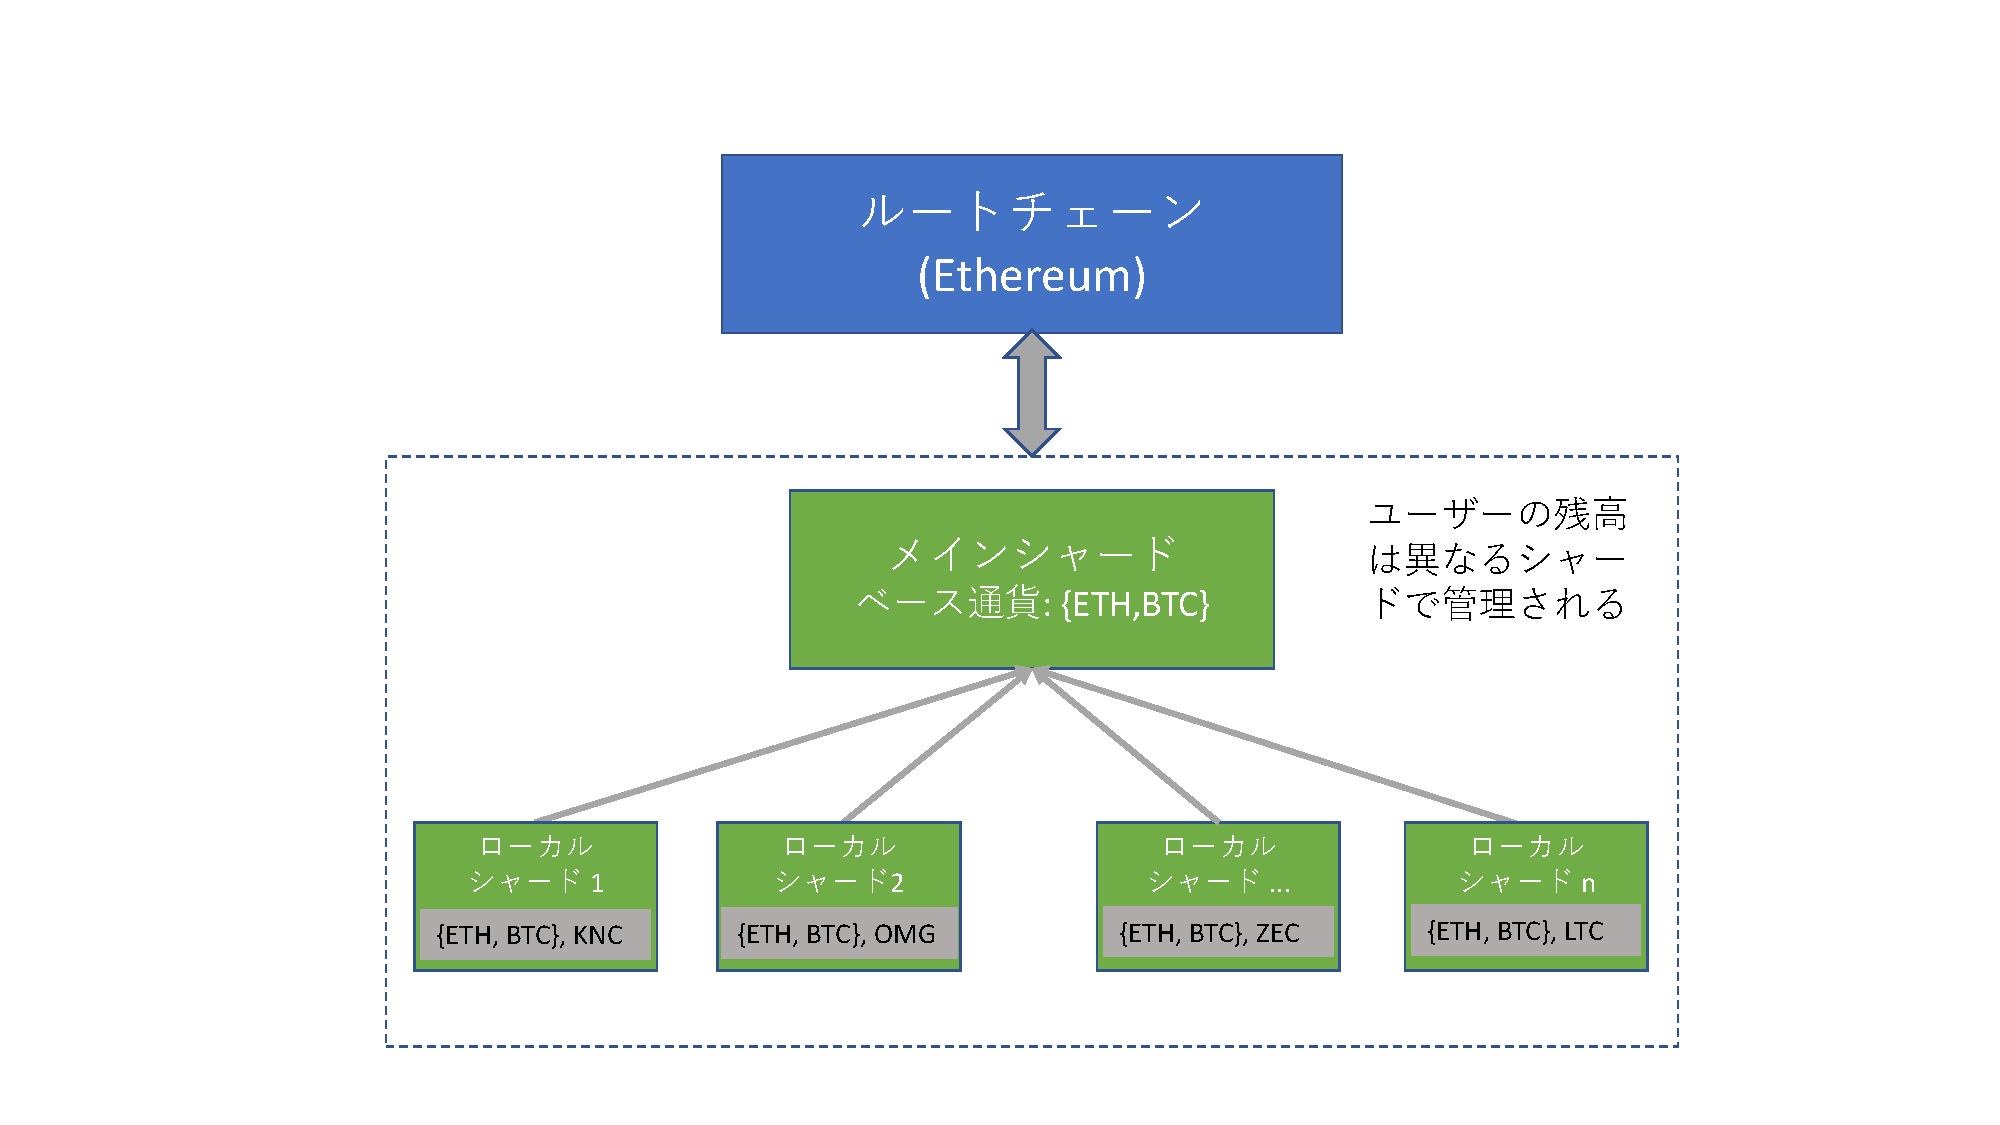
\includegraphics[width=0.8\textwidth]{images//architecture2}
  \caption{\codenameのデザインアーキテクチャ}
  \label{architecture2}
\end{figure}

シャード内のバリデーターは、フォールトトレラントなコンセンサスプロトコルを実行し、定期的にシャードのトークンペアの最新の取引に同意します。 具体的には、4〜5秒ごとにシャードバリデーターは、前のブロック以降のユーザーの取引注文を表す新しい取引を含む新しいデータブロックを発行します。 取引注文は、新規の売買注文や既存の注文のキャンセルがあります。 シャードに記録されたすべての取引要求に基づいて、バリデーターは、シャード内のこのトークンペアの完全な注文書を保持することができます。 バリデーターは、どの取引注文がマッチしているかを知ることができ、ユーザーの残高を更新するために決済を行うこともできます。 下の図は、ブロックデータの例と、ブロックが作成された後のユーザーの残高の変化を示しています。 第~\ref{sec:details}章では、取引注文フォーマットの詳細、シャード内のブロック構造について議論します。

\subsection{シャード・インスペクタ:チェーンのガーディアン}

パブリックブロックチェーンを中央集権的システムよりも魅力的にする優れた特性は、すべてが公に監査可能で検証可能であることです。公開鍵暗号のおかげで、不正または悪意のあるすべてのアクティビティについて、悪質なアクターに説明責任を持たせることができます。すなわち、悪質なアクターは、暗号学的証明を条件に何も間違っていないことを否定できません。そのため、誰でも、いつでも不正な行為が発生しているかどうかを検出するために公開ブロックチェーンのデータを観察し、悪質なアクターを特定することができます。 Plasmaでは、Plasmaチェーンを観察し、バリデーターによる不正行為があるかどうかを検出するためには、ユーザーがオンラインでなければならないという懸念があります。そうであれば、ユーザーは、fraud proofを提出してexitすることができます。これにより、自分の資産を取り戻し、バリデーターにペナルティを科すことができます。しかし、私たちの見解では、データが一般に公開されているので、この行動は誰でも行うことができます。第三者オブザーバーは、他のオブザーバーの代わりにexitすることができます。私たちは、この機能を拡張して、シャー​​ドインスペクタと呼ばれるすべてのシャードに新しいロール/プレイヤーを導入します。彼らの責任は以下の通りです。

シャード・インスペクタは、シャードのローカルコンセンサスに参加しておらず、単にシャードを観察して奇妙なことが起こっていないかを検証し、メインチェーン上にfraud proofを報告したり、シャードバリデーターを罰したりします。 シャード・インスペクタはデータの可用性も保証します。 彼らは、シャード内で生成されたすべてのデータブロックを保存し、ユーザーにデータを提供することができます。 これにより、シャード内のデータ可用性が向上します。 シャードインスペクタは、EthereumとBitcoinにおけるフルノードと考えることができます。ただし、これらのフルノードは上位機関に報告することで、マイナー(つまり、Plasmaチェーンのバリデーター)にペナルティを科すことができます。 以下のセクションでは、\codenameで実際にこの役割をどのように実施するか、そしてインスペクタに参加するようインセンティブを与える方法について詳しく説明します。

\subsection{相互運用性:多くのブロックチェーンをブリッジする}

既存の分散型取引所の大きな問題点の1つは、異なるコインと暗号通貨をサポートする能力です。 たとえば、BitcoinをEthereumに移行するためのシームレスな解決策が存在しないため、現在のユーザーは既存の分散型取引所でBitcoinと他のERC20トークンとの間で取引することはできません。\codenameがEthereumのエコシステム外で異なる暗号化通信をサポートするために使用すると考えるいくつかのソリューションとアプローチについて議論します。

\begin{itemize}

\item PeaceRelay: ユーザーはEVMベースの通貨をEthereumのメインチェーンと行き来することができます。 PeaceRelayは、2つのチェーン間の双方向リレーを構築し、ネイティブコインを1つのチェーンに固定して、Ethereum上のコインをトラストレスな方法で表現する新しいトークンを作成することを可能にします。 同様に、ユーザーはEthereum上で前記トークンをバーンして、他のチェーン上のコインを交換することもでます。 もちろん、PeaceRelayを使ってRootstock経由でBitcoinをEthereumに移動したり戻したりすることもできます。

\item Trustless Custodian approach: この最近提案されたソリューション~\footnote{\url{https://blog.kyber.network/bringing-bitcoin-to-ethereum-7bf29db88b9a}}は、ユーザーが簡単にBitcoinトークンを生成できるようにします。 それは、Bitcoinをデポジットするパブリックなウォレットを持っている保管人(必ずしも信頼できるとは限らない)です。 しかし、保管人はETHやEthereum上の他のトークンを担保にして、ユーザーは、Bitcoinを戻すためにバリデーターを報告してペナルティを科すことができます。

\item MakerDao’s approach: MakerDaoは、価値が1米ドルに固定された分散型ステーブルコイン(DAIなど)を構築するソリューションを設計しています。 ユーザーはETHを担保にしてDAIを発行することができ、担保付資産は常にDAIの全流通以上です。 MakerDaoは、担保付資産の総額を評価するためにETHの価格供給に依存しています。同じメカニズムを使用して、私たちはETHをBitcoinトークンを作成するための担保として使用し、ETH:Bitcoinの価格フィードに依存することができます。
\end{itemize}

\subsection{\codename: 高パフォーマンスな分散取引所}

これらのコア技術コンポーネントに基づいて、\codenameを高性能分散型取引所として構築します。\codenameが以下のようにすべての理想的な特性をどのように保管しているかを示します。

\begin{itemize}
\item スケーラブル. \codenameは、そのデザインに2つのスケーリングソリューション、すなわちPlasmaとシャーディングを実装しています。 Plasmaでは、高いスループットと安価(あるいは0)のトランザクション手数料を使用してルートチェーンからトランザクションを実行できますが、シャーディングでは、異なる取引ペアのアクティビティを分離することによって\codenameをスケールアップできます。
\item 低レイテンシ. \codenameの新しいブロックが作成されるとすぐに注文を確認することができます。これは、シャード設定に応じて4〜5秒以内に行うことができます。ただし、取引が最終化される、すなわちルート・チェーンにコミットされるまでには時間がかかることがあります。
\item セキュアで分散型. \codenameでは、バリデーターが悪意のある行為を行った場合に、ユーザーはサイドチェーンを終了し、資産をルートチェーンに戻すことができます。さらに、不正なバリデーターを報告し、罰則を科すfraud proofを提出することもできます。これにより、バリデーターが不正行為をするのを防ぐことができます。さらに、すべてのシャード内のコンセンサスは複数のバリデーターによって実行され、バリデーターはシャード間で頻繁にローテーションされるため、特定のシャード上でシャードを妥協したり、検閲を実施することは困難です。
\item 相互運用性. Bitcoinやその他の暗号化ツールをEthereumに移行するためのさまざまなアプローチにより、ユーザーは\codename上で異なる通貨ペアを取引することができます。
\end{itemize}

シャーディング・アーキテクチャーの優れた特性の1つは、トレーディング資産の明確な分離です。 その結果、異なるトレーディング資産のペアに対して専用のシャードを設けることができます。\codenameが特別なシャードを設けることで、人々はNFT(Non-Fungible Tokens)を交換することができます。また、ユーザーの参加に関する様々な要件を備えたセキュリティトークンの取引を容易にするために、特別な機関によって運営される別のシャードを設けることもできます。 たとえば、特別な機関のバリデーターが運用するシャード上でセキュリティトークンをサポートし、そのシャード上で取引を行うために、ユーザーの情報登録やKYCチェックを必須にすることができるでしょう。\codenameのシャーディング設計は、取引活動のダイナミックで明確な分離を可能にし、異なるプラットフォームを同じプラットフォームで共存させることを支援します。

\section{技術的な詳細}
\label{sec:details}

このセクションでは、バリデーターの選択方法、シャードの形成方法、シャッフル方法、\codenameでの取引の詳細について説明します。

\subsection{バリデーターの登録}
\codenameのバリデーターになるためには、KNCをルートチェーン(Ethereum)にデポジットしなければなりません。デポジットがPlasmaチェーン上で認識された後、バリデーターとして登録され、バリデーションプロセスを開始することができます。 バリデーターのデポジットの量を決定する方法はいくつかあります。 1つの方法は、量を固定し、いくらでもバリデーターを受け入れる方法です。 その結果、\codenameには何万人ものバリデーターがいるかもしれません。 もう1つのアプローチは、バリデーターになるためのデポジット額の決定は公開市場に任せて、固定数(たとえば1,000)のアクティブバリデーターのみを許可する方法です。この場合、 新しいアクティブバリデーターになるためには、現在のアクティブバリデーターリストの最低デポジットより多くのデポジットを入れなければなりません。最低金額のバリデーターは、たとえば24時間後に無効になります。ダイナミックデポジットは、バリデータスロットがどれくらいの価値があるか、プラットフォームにどれくらい信用があるかを市場が自由に決めることを可能にします。(バリデータの主なコストは機会費用です)

\subsection{シャード形成}
アクティブなバリデーターのリストから、\codenameはバリデーターをさまざまなサブセットに配布し、それぞれがシャードを担当します。 一般に、$N$をバリデーターの数とし、$n$をシャード数とし、各シャードに$c$バリデーター(したがって$N = n*c$)を持たせます。 より多くのシャード(より多くの$n$)がある場合、よりアクティブなバリデーターを受け入れ($N$を増やす)、新しく作成されたシャードの異なる取引ペアをサポートすることができます。 理想的には、VRF~\cite{algorand}やRandHound~\cite{randhound}などで実現できる偏りのないグローバル乱数ジェネレータに依存する一様分布を作りたいと考えています。 しかし、不正なバリデーターが行うことができる最も大きな損害は、シャードで検閲を行うこと、またはファイナライズされていない取引をなかったことにすることであるため、潜在的なバイアスが小さい乱数のソースを用いることができます。 \codenameの最初のイテレーションでは、ルートチェーンのブロックハッシュをランダムシードとして使用することを提案します。

より良い決済レイテンシを達成するためには、シャード内のコンセンサスは、小さな数$c_c$以内のバリデーターによってなされなければなりません。 たとえば、シャード内のローカルブロック時間を2秒にするには、以前の実験~\cite{elastico}に基づいて、$c_c$は約20でなければなりません。しかし、シャード内のバリデーターの数$c$は、数百に上げることができます。すなわち、シャード内のバリデーターには2つの異なるロールがあります。

\begin{itemize}
\item シャードコンセンサスバリデーター: シャードには、新しいトランザクションの検証と新しいブロックの生成に積極的に関与する$c_c$個のバリデーターが存在します。
\item シャード・インスペクタ: 前述したように、残りのバリデーターはシャード・インスペクタであり、シャード内のフルノードのように動作します。 これらは、シャードの完全な状態を保存し、データの可用性を保証します。
\end{itemize}

バリデーターに対する標的攻撃を軽減するために、\codenameは定期的にシャード・インスペクタをシャード内の新しいコンセンサス・バリデーターに昇格させ、既存のコンセンサス・バリデーターをシャード・インスペクタとして機能する新しいシャードに再配置します。 昇格と再配置のプロセスも、前述のグローバル乱数ジェネレータに依存する統一された方法で行われます。

\begin{figure}[t]
  \centering
  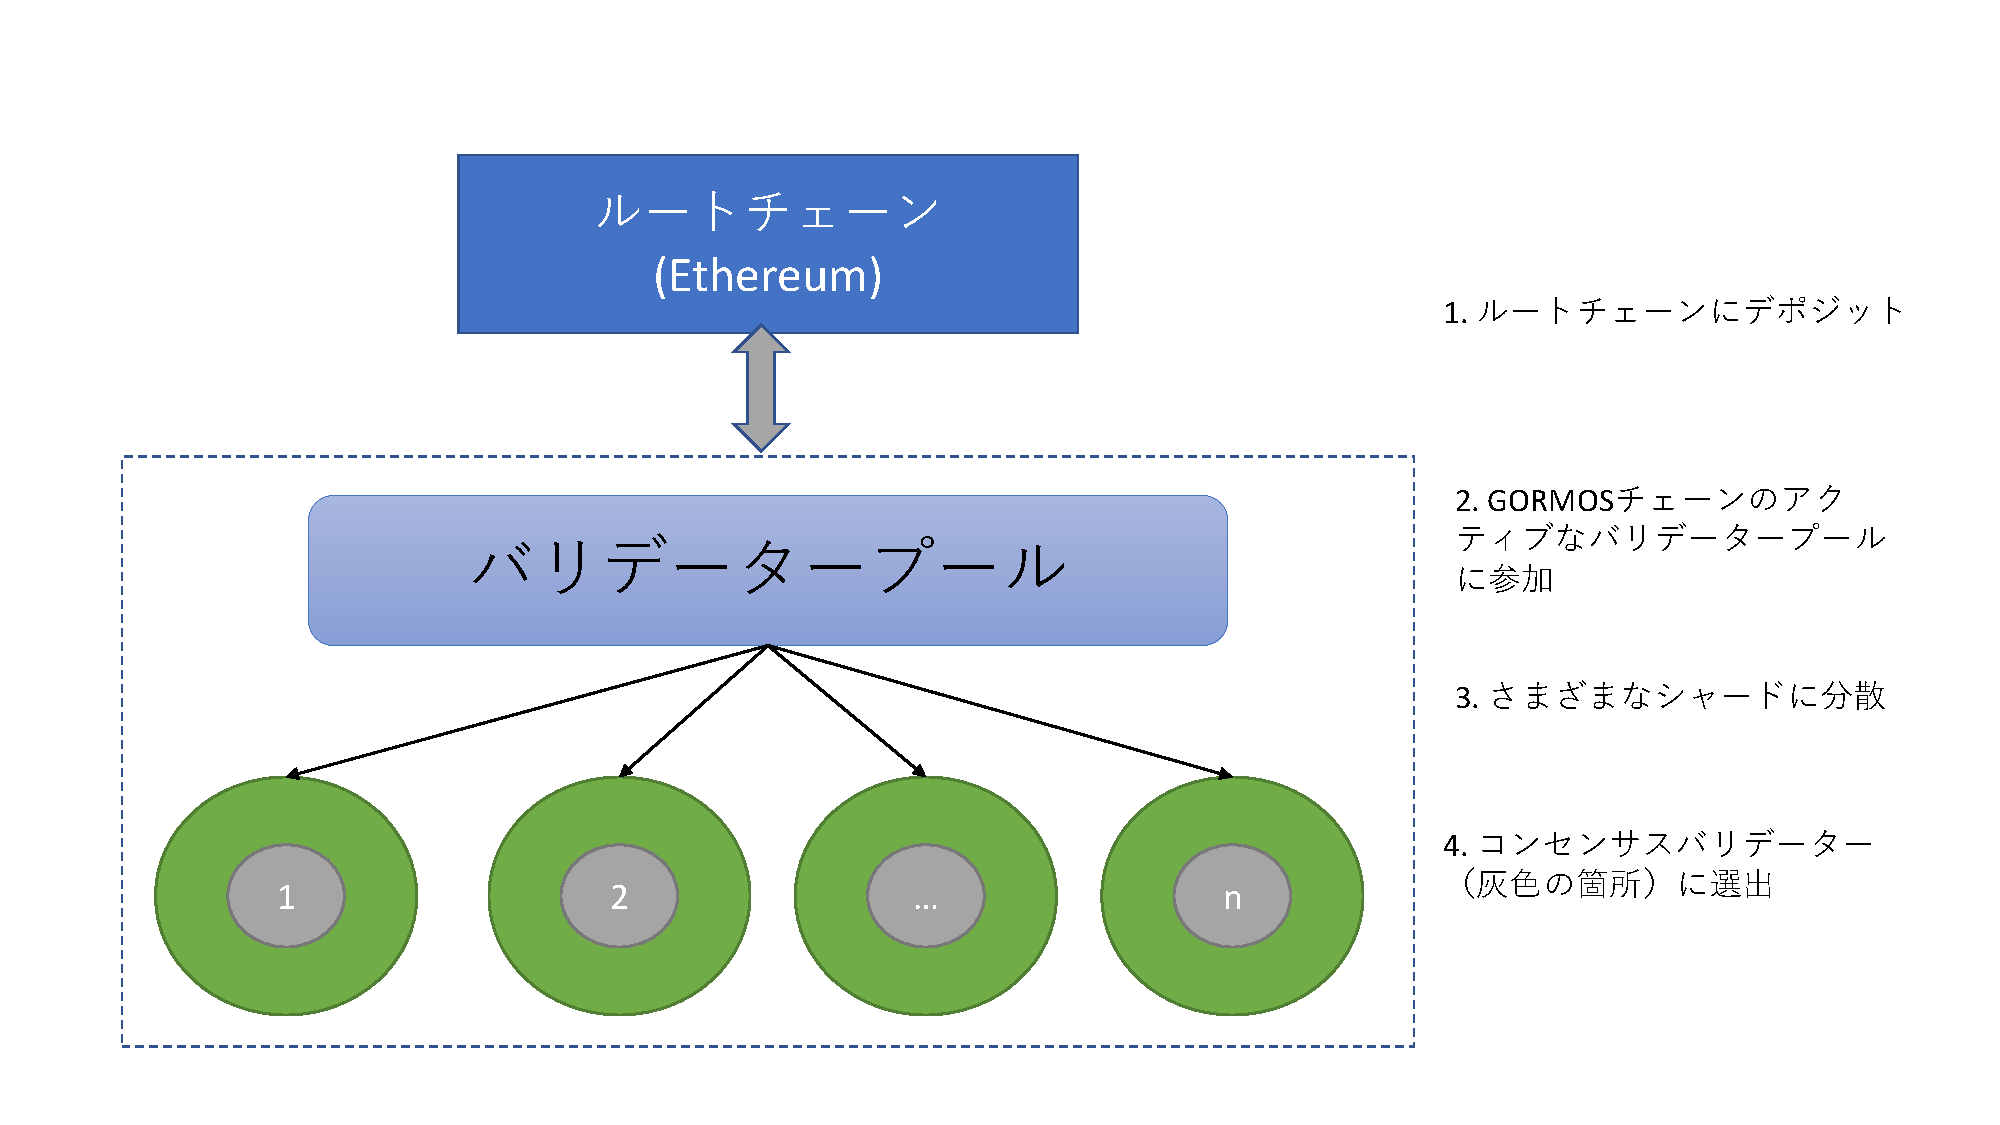
\includegraphics[width=0.8\textwidth]{images/validator}
  \caption{\codename においてバリデーターになるためのステップ}
  \label{fig:validator}
\end{figure}

\subsection{取引の実行とブロックフォーマット}

\textbf{取引フォーマット.} \codenameのユーザーは、トランザクションを
シャード シャード内のトランザクションは、以下の情報で構成されます。
\begin{align*}
(\mtt{addr}, \mtt{shard\_id}, \mtt{src\_token\_id}, \mtt{des\_token\_id}, \\ \mtt{order\_type}, \mtt{src\_amount}, \mtt{fee}, \\ \mtt{metadata}, \mtt{nonce}),
\end{align*}

ここで、
\begin{itemize}
\item $\mtt{addr}$: ユーザーのアドレス
\item $\mtt{shard\_id}$: ユーザーが取引をしているシャードのID
\item $\mtt{src\_token\_id}$: ユーザーが取引元にしたいトークンのID
\item $\mtt{des\_token\_id}$: ユーザーが取引先にしたいトークンのID
\item $\mtt{order\_type}$: リミットオーダーやマーケットオーダー、既存オーダーのキャンセルリクエストなど
\item $\mtt{src\_amount}$: ユーザーが取引したいソーストークンの量
\item $\mtt{fee}$: ユーザーが支払おうとした手数料(\%)(トランザクション手数料と同様)
\item $\mtt{metadata}$: 注文に関する詳細なデータ。たとえば、$\mtt{order\_type}$がリミットオーダーの場合、ユーザーは価格を含める必要があり、注文タイプがキャンセルリクエストの場合、$\mtt{metadata}$は$\mtt{order\_id}$を持ちます。これは、以前の注文のハッシュです。
\item $\mtt{nonce}$: Ethereumのトランザクションnonceに似ています。これは、これまでにユーザーが作成したオーダーの数です。
\end{itemize}

\textbf{ブロックフォーマット.} \codenameには、ローカルデータブロックとメインブロックという2つのブロックがあります。 シャード内のローカルデータブロックは、生の新しいトランザクションデータと、次のフィールドを持つデータブロックヘッダーで構成されます。

\begin{align*}
(\mtt{shard\_id}, \mtt{block\_number}, \mtt{prev\_block\_hash},\\ \mtt{new\_order\_merkle\_root}, \mtt{balance\_merkle\_root}, \mtt{avail\_balance\_merkle\_root},\\ \mtt{open\_order\_MMR\_root}, \mtt{closed\_order\_MMR\_root}, \mtt{cancelled\_order\_MMR\_root},\\ \mtt{timestamp}, \mtt{signatures}),
\end{align*}

ここで、
\begin{itemize}
\item $\mtt{shard\_id}$: ユーザーが新しい注文で取引をしているシャードのID 
\item $\mtt{new\_order\_merkle\_root}$: このブロックのすべての新しい注文をコミットするMerkleルート
\item $\mtt{balance\_merkle\_root}$: このブロック内のすべての新しい注文を受け入れた後、シャード内の全員の残高をコミットするMerkleルート  
\item $\mtt{avail\_balance\_merkle\_root}$: このブロック内のすべての新しい注文を受け入れた後、シャード内の全員の利用可能な残高をコミットするMerkleルート
\item $\mtt{open\_order\_MMR\_root}$: このシャードのすべての未処理注文をコミットするMerkle Mountain Rangesルート
\item $\mtt{closed\_order\_MMR\_root}$: このシャード内のすべてのクローズ注文をコミットするMerkle Mountain Rangesルート
\item $\mtt{cancelled\_order\_MMR\_root}$: このシャードのすべてのキャンセル注文をコミットするMerkle Mountain Rangesルート 
\end{itemize}

一方、メインブロックはローカルシャードのすべてのローカルブロックヘッダを格納し、その結果を単一のメインブロックヘッダに合成します。 たとえば、メインブロックのブロックヘッダは、以下のようにすることができます。

\begin{align*}
(\mtt{block\_number}, \mtt{prev\_block\_hash}, \mtt{new\_local\_headers\_merkle\_root}, \\ \mtt{new\_order\_merkle\_root}, \mtt{balance\_merkle\_root}, \mtt{avail\_balance\_merkle\_root}, \\ \mtt{open\_order\_MMR\_root}, \mtt{closed\_order\_MMR\_root}, \mtt{cancelled\_order\_MMR\_root},\\ \mtt{timestamp}, \mtt{signatures}),
\end{align*}
すべての新しいMerkleルーツはローカルブロックのヘッダーからのMerkleルーツに基づいて計算されます。

\textbf{Merkle Mountain Rangeの活用.}  Merkle Mountain Rangeを活用して、閉鎖されたすべての注文、発注、キャンセルされた注文などのブロックごとにMerkleツリーを効率的に更新できるようにします。 \codenameは、最近提案されたデータ構造(Merkle mountain range(MMR))を利用して、軽いクライアントが最新のブロックのみでブロックチェーン上の任意のイベントを効率的に検証できるようにします。
MMRを使用すると、すべての前のブロックを1つのハッシュで最新のブロックヘッダーに効率的にコミットできます。もちろん、元のMerkleツリー構造をそのまま使用して同じ目標を達成することはできますが、Merkleツリーを新しいブロックヘッダーで更新することは効率的ではありません。 Merkleツリー全体を再構成するか、または$\log{n}$ハッシュよりもはるかに大きい証明サイズをもたらす「アンバランス」ツリーに苦しむ必要があります。 MMRは、より効率的な更新プロセスを可能にする元のMerkleツリーの変形であるため、ブロックを処理する際の完全なノードのオーバーヘッドは無視できる程度になります。

\subsection{シャード内のコンセンサスプロトコル}\label{shard-consensus}
Plasmaでは、Minimal Viable Plasma~\cite{plasma-mvp}やPlasma Cash~\cite{plasma-cash}で示唆されているように、Proof of Authorityのような集中型コンセンサススキームに頼ってセキュリティを犠牲にすることはありません。 しかし、フォールトトレランスとセンサー耐性を向上させるために分散化が必要なため、合理的に多数のバリデーターを実行するために各シャードで効率的なBFTプロトコルを選択します。 たとえば、非同期ネットワークで高スループット(64ノードで$\approx 1.2*10^4\hspace{3pt} tx/s$)を達成するHoneyBadger BFT\cite{honeybadger}が良い候補です。

\textbf{Practical asynchronous BFT in sporadic layer-2 network}.
シャード内のバリデーターは、ルートチェーン内の基礎となるネットワークから分離された別のP2Pネットワークで動作しなければならなりません。私たちの目標は、ネットワークが許す限り速く、平均で2秒のブロック時間で、シャードが新しいブロックを提案できるようにすることです。 異なるシャード内のブロックは、非同期方式で生成されます。すなわち、異なるシャードは、異なる速度でブロックをファイナライズし、メインシャードは、メインブロックを生成するときに、利用可能なすべてのローカルブロックをみます。そこで、HoneyBadger BFT~\cite{honeybadger}で提案された最適化を用いた非同期アトミックブロードキャストプロトコルと非同期共通サブセットのより効率的なインスタンス化を目的とした公開鍵暗号化を利用する予定です。

\subsection{Fraud proofの提出とexit}
ここでは、何か悪意のある事態が発生した際に、ユーザーがどのようにfraud proofをルートチェーンに提出し、\codenameチェインを正常にexitするのかにについて説明します。 シャード・インスペクタによってデータの可用性が維持されていると仮定すると、2つのケースが考えられます。1つは、シャード内の共謀バリデーター(および機能しないインスペクター)が不正なトランザクション(有効なシグネチャまたは入力のミスマッチ、出力量)を取り込んだ場合、 もう1つの可能性は、ネットワーク障害や攻撃者の意図的なメッセージのドロップにより、ネットワークの非同期が発生し、シャードが正常に進まなくなってしまった場合です。

ユーザーはフルノードにリクエストを送信することでfraud proofを取得します。フルノードは、シャード・インスペクタまたは自分自身(ユーザーがフルノードを実行している場合)になります。 ユーザーの送信する要求では、ユーザーが正しいと合意する特定のブロックを指定します。つまり、そのブロック以降の他のブロックは無効と見なされます。フルノードからの応答は、その特定のブロック高での状態ツリーのユーザーバランスのMerkle Proofです。ユーザーはインフォーマルに次のような主張を行います。「私の最新の残高としてこのブロックの残高に同意します。次のブロックに不正な署名が含まれているか、動作が停止しているためにexitしたいと思います。」

最初のシナリオでは、ユーザーは2つのMerkleパスをルートチェーン(Ethereum)に提出します。1つは状態ツリー内の最新の有効な残高のMerkleパスです。もう1つは悪意のあるバリデーターによって偽造された無効な状態のパスです。Plasmaのメインシャードの定期的なコミットにより、ルートチェーンは提出されたMerkle Proofを検証し、証明が有効になるとチャレンジ期間を開きます。 この期間中、悪意のあるバリデーターが、ユーザーからの正式な署名を使用して、前者から後者への状態遷移を示す有効なトランザクションを提供できない場合、バリデーターは処罰され、その預金は失効し、ユーザーは最後の有効な残高でexitすることができます。

2番目のケースでは、そのシャード内の各ユーザーが1人ずつ退出することもできます。これは、チェーン上のすべての決済であるため、非常に高額です。 オンチェーンのメッセージ数を減らすために、Plasmaで提案されているmass withdraw手法を用いることができます~\cite{plasma}。\codenameが提供する優れた特性は、1つのシャードからexitすることが残りのシャードに影響しないことです。 ダメージが独立しているため、\codenameの設計はより堅牢です。

\subsection{バリデーターのインセンティブ}
バリデーターになる主なインセンティブは、シャード内の処理済みの取引すべてから取引手数料を得ることです。これはコンセンサスラウンドに参加するバリデーターにとってより明白です。続いて、そのシャードのフルノードデータを保存し、シャードの中に何らかの不具合が起きたかどうかを監視するシャード・インスペクタのインセンティブについて議論します。

まず、シャード・インスペクタは、同じシャード内の次のラウンドのバリデーターの適格候補です。なぜなら、インスペクタが保持しているすべてのデータがなければ、新しい今後のトランザクションを検証することは不可能だからです。加えて、シャード・インスペクタだけが、シャードのコンセンサスに参加するために選ばれます。

第二に、シャード・インスペクタが不正行為を発見したら、ユーザーのためにfraud proofを提出し、失効した預金から報酬を得ることができます。ほとんどの場合、シャード・インスペクタはつねにオンラインであり、ユーザーよりも厳密にシャードを監視しているため、不正を発見できる機会は多いでしょう 。さらに、インスペクター/フルノードとして、(コンセンサスバリデーターと比較して)取引手数料のほんの一部を受け取ることもできます。

\subsection{他のユースケースのための\codename}
\label{sec:others}

分散型取引所以外のアプリケーションで\codenameを使用して、オンチェーンでより多くのトランザクションをスケーラブルかつ低レイテインシで実行できるようにする方法について説明します。第~\ref{sec:intro}章で説明したように、\codenameのスケーラビリティは、アクティビティを異なるシャードに分けることによってもたらされます。その結果、\codenameは、別々のコンポーネントを持つアプリケーションに適しており、これらのコンポーネント間の相互作用はあまりありません。たとえば、Etheremonはポケモンに似たゲームで、ユーザーは "モンスター"を育成して成長させ、他の人と競うことができます。モンスターは、ゲームマップの異なる場所に属する異なる「ジム」に移動することができます。 \codenameを使用すると、Etheremonはマップを異なるシャードに対応する異なるローカルマップに分割することができ、各シャードはゲーム内の地理的領域を表します。シャードは、それぞれのローカルマップ内のすべてのモンスターと活動を管理します。ユーザーは、メインのシャードにトランザクションを送信して、自分のモンスターに存在する新しいローカルマップを示すことによって、モンスターを異なるローカルマップに移動できます。 Etheremonのほとんどのアクティビティがジム内で起こるか、モンスターが同じ地域でのみ出会えるとき、\codenameは間違いなくユーザーエクスペリエンスに影響を与えずにEtheremonをスケールアップする最良の設計です。

同様に、すべての旅行、支払い、格付けがチェーン上に記録されている分散Uberのような他のユースケースには\codenameを使用できます。
\codenameベースのUberは、異なるシャードを持つことができ、それぞれが都市を担当します。シャード内のバリデーターは、都市内のすべてのトランザクションを検証し、ローカルブロックに組み込みます。一般的に、地理的に分散されているか、またはアーキテクチャ上異なるコンポーネントに分かれているアプリケーションは、\codenameの恩恵を受けることができます。

\section{Governance and Token Utility}
There are a few parameters that could be subjected to on-chain governance through stake-based voting. Each of these voting scenarios will be a set of functions implemented smart contracts on either the root-chain or on \codename.

\begin{itemize}
\item Token pairs add/delete: adding a new pair involves creating a new shard and potentially either increase the validator pool or temporarily delute the number of validators per shard. Similarly, when certain shard is inactive or not having enough activity, stakeholders in this plasma chain could vote to drop this shard or merge it with existing shards.

\item Validator registration threshold: this should be amenable based on the community's confidence in the comparison between their security deposit and the amount of transactions these validators are securing. ( by default, there should be a minimum barrier specified, and any further governance decision could only move around this parameter above this floor) 
\item Validators Pool: change the number of validators chosen for each shard.

\end{itemize}
\textbf{Token Utilities.} KNC or any underlying token of \codename can be used for several utilities, including but not limited to the follows.
\begin{itemize}
\item Staking to be \codename validators. This is a basic staking function that requires validators to deposit KNC to the main \codename's contract in the root chain (i.e. Ethereum).
\item Using KNC to pay for trading fees and get discount. This utility is used in several popular exchanges including Binance, Huobi. This can be implemented easily on \codename.
\end{itemize}

\section{Future Work}
This paper focused on the architectural design and system properties of \codename, which
leverages on careful interplay multiple state-of-the-art scalability solutions to build a
high performance decentralized exchanges on cryptocurrency systems. The open question that is left for future work is
 how to deal with front running. Miner/validator frontrunning is a well-observed
  problem in permissionless blockchain system and is particularly troubesome in auction system
  and exchange market. Specifically in \codename design, validators in each shard are able to profit from
  "front running" the original order takers by pushing their own filling transactions first and resell later
  at a higher price due to change in liquidity. Proposals like \textit{Submarine Send}\cite{submarine}
  utilizes improvised "Commit-Reveal" paradigm where commit (also called "submarine send") is indistinguishable
  from a normal transaction thus indistinguishable from miners' perspective, given sufficient anonymity-set size. It is
  a viable solution for auction bid and order fill. However, it is still not clear how Submarine prevents validators from committing a lot of fake orders and only reveal the one that benefits them to front-run some specific order. In addition, this solution affects usability as it will introduce delay (confirmation blocks between commit phase
  and reveal phase) and users will have to take extra steps to participate in the protocol. 
  Note that on centralized exchanges, front-running is easier to do, and its hard to even detect if the exchange is front running other users.

\section{Acknowledgment}
We thank our advisors Prateek Saxena, Vitalik Buterin and Patrick McCorry for useful discussions and feedback on the early version of
the paper.


\bibliographystyle{styles/splncs03}
\bibliography{paper}

% \appendix
% \input{appendix.tex}
\end{document}
